\chapter{Der Berkeley Data Analytics Stack (BDAS)}
\label{chapter:grundlagen des BDAS}


Rund um \textit{Hadoop} beziehungsweise \textit{Spark} wurde an der University of California in Berkeley ein ganzer Infrastruktur-Stack für Big-Data-Analytics aufgebaut, der BDAS. Im folgenden Kapitel wird dieser Stack und die Bibliotheken, aus dem dieser besteht, vorgestellt. Im ersten Unterkapitel wird zunächst ein kurzer Überblick über den gesamten Stack gegeben. In den darauffolgenden Unterkapiteln werden die einzelnen Bestandteile im Einzelnen oberflächlich betrachtet, um dem Leser einen Einblick in die Nutzungsmöglichkeiten zu bieten. Eine Detailbetrachtung der jeweiligen Grundlagen, der praktischen Anwendung, Messungen und Vergleichsbetrachtungen der Alternativimplementierungen folgen im weiteren Verlauf dieser Ausarbeitung. Das Kapitel schließt mit einer Zusammenfassung, die auf einen Blick die Zusammensetzung des BDAS rund um Apache Spark zeigt. 


\section{Die Schichten des BDAS}
\label{section:schichten des BDAS}

	
	Im Folgenden wird der \textit{Berkeley Data Analytics Stack (BDAS)} näher vorgestellt, der wie in der Einführung bereits erwähnt um Hadoop, bzw. Spark als Hauptbestandteile herum aufgebaut ist. Der BDAS wurde von den \textit{AMPLabs} \footnote{kurz für „algorithms, machines and people“} von der University of California in Berkeley aufgrund von Forschungsergebnissen im Bereich der Analyse sehr großer Datenmengen ins Leben gerufen. 

Der Einsatz des BDAS kann laut Vijay Agneeswaran \citelit{va14} dabei helfen, beispielsweise konkrete praktische Fragen wie die folgenden zu beantworten: 

\begin{itemize}
		\item Wie segmentiert man am besten eine Menge von Nutzern und kann herausfinden, welche Nutzersegmente an bestimmten Kampagnen interessiert sein könnten?
		\item Wie kann man richtige Metriken für Nutzer-Engagement in Social-Media-Applikationen herausfinden?
		\item Wie kann ein Video-Streaming-Dienst für jeden Nutzer dynamisch ein optimales \textit{Content-Delivery-Network (CDN)} \footnote{Ein Content Delivery Network (auch Content Distribution Network) ist ein Netzwerk verteilter und über das World Wide Web verbundener Server, das den Zweck hat, grosse Dateien bereitzustellen und auszuliefern.} basierend auf Daten wie Bandbreite, Auslastung, Pufferrate, etc auswählen?
		
\end{itemize}	


Prinzipiell sind die in der Einführung in Kürze beschriebenen Einschränkungen von Hadoop und die damit verbundene Motivation für Spark auch die Motivation für den BDAS. Besonders für Aufgaben, die iterative Datenzugriffe und -manipulationen erfordern, wie beispielsweise Machine-Learning Algorithmen oder interaktive Abfragen, ist Hadoop auf Grund seiner starken festspeicherabhängigkeit nur bedingt zu empfehlen. Für diese Aufgaben ist Spark mit seinen In-Memory-Primitives prädestiniert. Um Hadoop herum ist in den letzten Jahren ein umfangreiches Ökosystem von Bibliotheken und Frameworks gewachsen, so dass die meisten Aufgaben im Umfeld von Big-Data-Analytics mit einer Hadoop-Infrastruktur gelöst werden können. Dagagen spricht laut \citelit{dz14}, dass für jeden Nutzungsfall ein eigener, auf Hadoop basierender Technologiestack eingesetzt werden muss, große Expertise in mehreren Technologien für produktives Arbeiten nötig ist und die Architektur vor allem für Aufgaben, bei denen schneller Datenaustausch zwischen parallel bearbeiteten Tasks notwendig ist, unpassend ist. 

Im Gegensatz dazu bietet der BDAS auf allen Ebenen Standard APIs für Java, Scala, Python und SQL an und mit MLLibs stehen etliche Machine-Learning-Alogrithmen direkt in Spark zur Verfügung. Der Stack obehalb von Spark ist flexibel konfigurierbar und sämtliche Bibliotheken lassen sich parallel betreiben. 


In Abbildung \ref{fig:BDAS1} wird eine Übersicht über die Hauptschichten des BDAS gezeigt, welche die jeweils von den AMPLabs empfohlene Implementierung zeigt.

\begin{figure}[htb!]
\centering
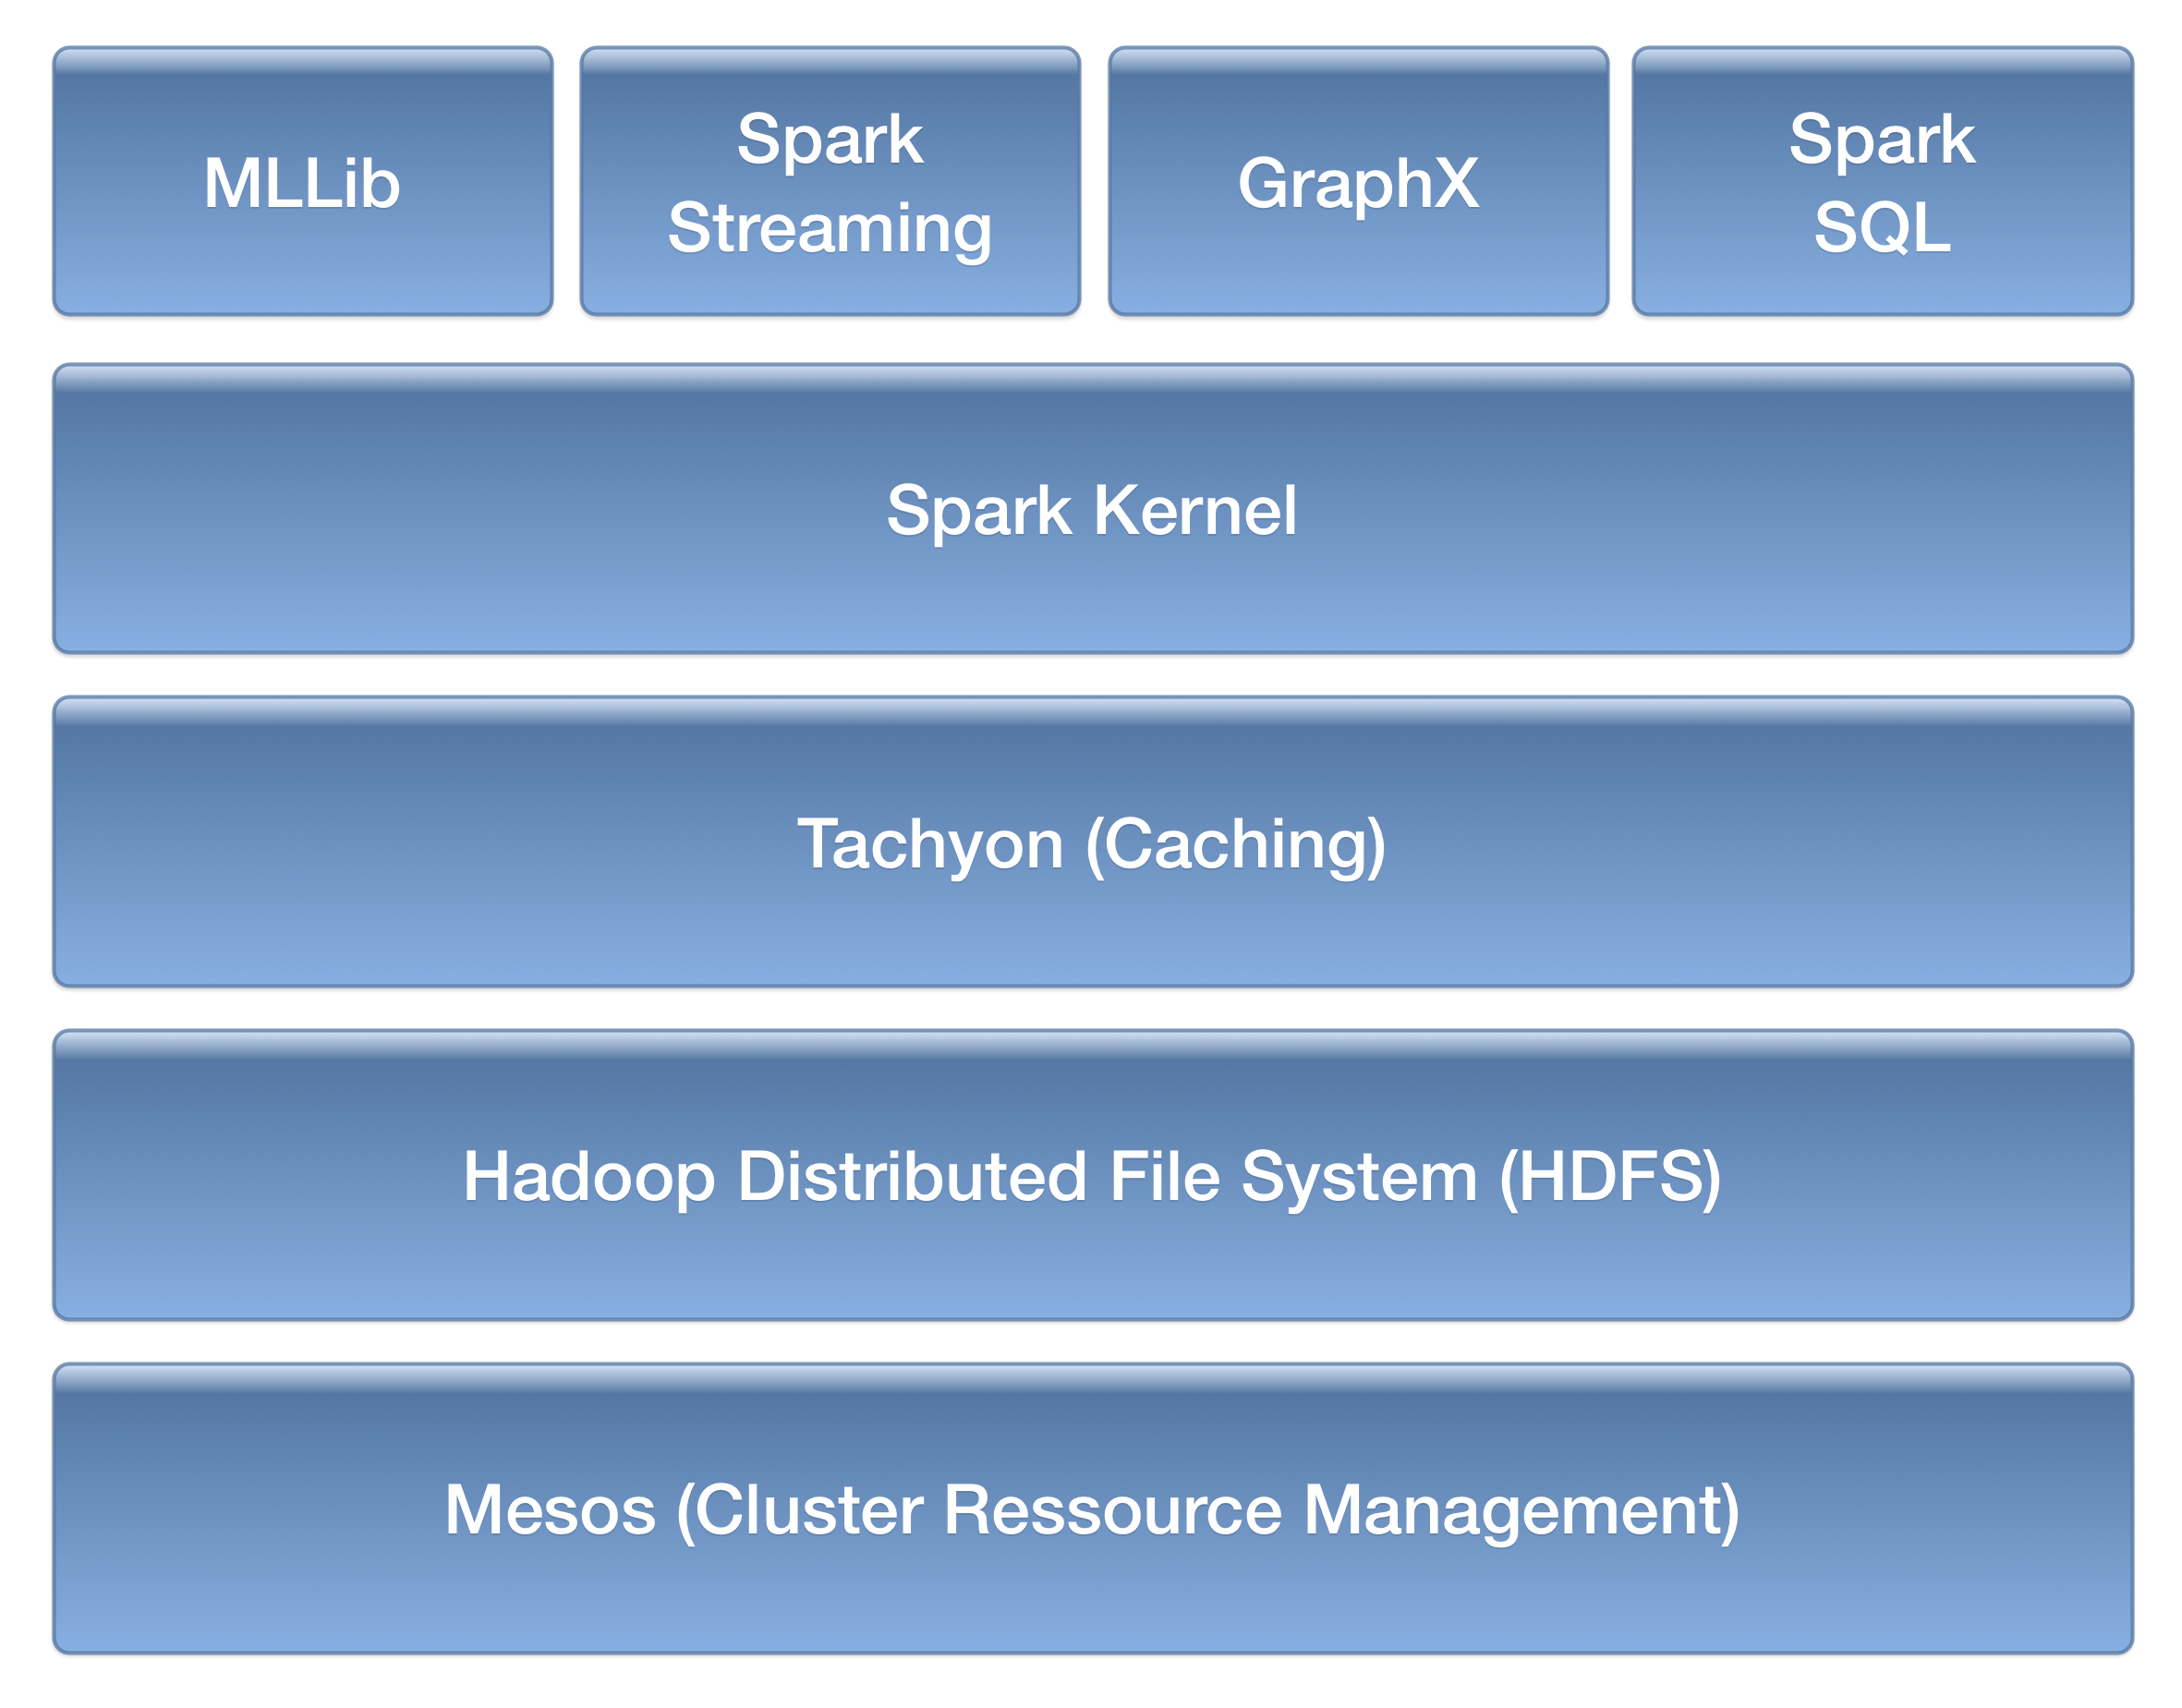
\includegraphics[width=1.0\textwidth]{bilder/BDAS.png}
\caption{Übersicht des BDAS mit den vom AMPLab empfohlenen Bibliotheken.}
\label{fig:BDAS1}
\end{figure}
 
In der untersten Schicht befindet sich das Cluster-Management-System Mesos, darüber das verteilte Filesystem HDFS, die Caching-Schicht Tachyon und der eigentliche Spark Kernel. Auf diesem setzen die Bibliotheken MLLib für Machine-Learning, Spark Streaming für Streaming-Anwendungen, GraphX für Graphenanwendungen und für datenbankähnliche Abfragen auf dem BDAS Spark SQL auf. 

In den folgenden Unterkapiteln werden die einzelnen Elemente des BDAS detailliert vorgestellt.   
\newpage

\section{Apache Mesos}
\label{section:apache Mesos}


Bei \textit{Apache Mesos} handelt es sich um ein \textit{Cluster-Management-Framework} für Anwendungen, die in verteilten Serverpools laufen sollen. Bestandteil von Mesos ist wiederum \textit{Apache ZooKeeper}, das für Konfigurationsinformationen, Naming-Services und die Synchronisation von verteilten Anwendungen zuständig ist.  

Mesos wird im BDAS eingesetzt, um die Prozesse von Hadoop/Spark effizient auf die einzelnen Knoten im Cluster zu verteilen. Besonders das Ressourcen-Management und –Monitoring innerhalb des Clusters ist ein wichtiger Faktor, um Jobs performant auf verteilten Systemen ausführen zu können. Auch das Fehlerhandling für Knoten, Prozesse und im Netzwerk wird im Berkeley-Stack von Mesos übernommen. 

Ein besonderer Vorteil von Mesos gegenüber Yarn oder anderen Alternativen, wie dem Cloudera Cluster Manager oder Ambari von Hortonworks ist die Möglichkeit, verschiedene Frameworks gleichzeitig und isoliert in einem Cluster betreiben zu können. So kann beispielsweise Hadoop mit Spark in einer gemeinsamen Infrastruktur koexistieren.   
	
\section{Hadoop Distributed File System (HDFS) und Tachyon}
\label{section:hadoop Distributed File System (HDFS) und Tachyon}


Das Hadoop Distributed File System basiert ideologisch auf dem GoogleFileSystem (GFS) und hat zum Zweck, zuverlässig und fehlertolerant sehr große Dateien über verschiedene Maschinen hinweg in verteilten Umgebungen zu speichern. In entsprechenden Veröffentlichungen von Hortonworks \citeint{ho14} wird von Produktivsystemen berichtet, die bis zu 200 PetaByte an Datenvolumen in einem Cluster von 4500 Servern basierend auf HDFS verwalten.

HDFS wurde speziell für den Einsatz mit MapReduce entwickelt, ist also auf geringe Datenbewegungen ausgelegt, da MR die Berechnungsprozesse jeweils zu den physischen Datensätzen selbst bringt und nicht, wie herkömmlich, die Daten zu den Prozessen geliefert werden müssen. So wird massiv Netzwerkverkehr innerhalb des Clusters eingespart und letztlich werden nur Prozesse und Prozessergebnisse verschickt.  

Die Hauptbestandteile von HDFS sind der sogenannte NameNode, der die Metadaten des Clusters verwaltet und die DataNodes, die die eigentlichen Daten halten. Dateien und Verzeichnisse werden vom NameNode durch inodes repräsentiert. Diese wiederum enthalten Informationen über Zugriffsrechte, Zugriffszeiten oder Größenangaben der Dateien.



\begin{figure}[htb!] 
\centering
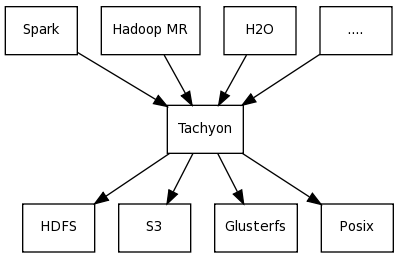
\includegraphics[width=1.0\textwidth]{bilder/2_3_stack.png}
\caption{Der Datamanagement-Layer im BDAS mit Tachyon und diversen Filesystemen \protect\citeint{tac14}.}
\label{fig:datamgmtlayer}
\end{figure} 

 

In Abbildung \ref{fig:datamgmtlayer} wird die Datenmanagementschicht des BDAS detaillierter dargestellt. Es lässt erkennen, dass zwischen den Frameworks und dem Data-Layer ein optimiertes Caching-Framework für sämtliche Dateisystemaufrufe zum Einsatz kommen kann.  

Hier lässt sich wahlweise direkt das \textit{HDFS} bzw. dessen Alternativen ansprechen oder alternativ die Zwischenschicht nutzen, die insbesondere auf das In-Memory-Modell von Spark zugeschnitten ist. Dies ist innerhalb des BDAS das verteilte Dateisystem Tachyon. Hier werden die zu verarbeitenden oder zu analysierenden Datensätze direkt in den Hauptspeicher des jeweiligen Knoten in Form eines Cache gehalten. Somit werden Lade- und Speicheroperationen auf Massenspeicher minimiert und eine massiv höhere Ausführungsgeschwindigkeit erreicht.

Tachyon besteht aus einem Master, der in der Regel dem physischen Master einer Spark-Infrastruktur entspricht. Dieser deligiert und überwacht die einzelnen Tachyon Worker-Nodes, die auch den Spark Worker-Nodes entsprechen. Tachyon implementiert auf jedem Knoten ein eigenes RAM-Filesystem, das den Hauptspeicher abseits des JVM-Heaps nutzt \citeint{tah14}.

Unterhalb von Tachyon ist nach wie vor ein HDFS für die persistente Datenhaltung notwendig. Alternativ kann auch das Amazon S3-File-System, Glsuterfs oder Posix eingesetzt werden. Tachyon wurde direkt innerhalb der AMPLabs entwickelt und ist mittlerweile fester Bestandteil des BDAS.  


\section{Apache Spark}
\label{section:apache Spark}

Spark ist das Herzstück des BDAS. Bei Spark handelt es sich um ein open-source Data-Analytics-Framework, das, wie Hadoop, speziell für die Bedürfnisse im Rechner-Cluster konzipiert ist. Auch Spark nutzt das HDFS entweder direkt, oder indirekt über Tachyon. Im Gegensatz zu Hadoop bietet Spark jedoch Funktionen für In-Memory-Cluster-Berechnungen und ist nicht zwingend an MapReduce gebunden. Besonders interaktive Analyse oder Verarbeitung der Daten, Abfragen über verteilte Dateien und iterative 

Lernalgorithmen erfahren so laut AMPLab eine bis zu hundertfache Ausführungs-geschwindigkeit im Gegensatz zu Hadoop. Auch die im ersten Kapitel angesprochenen Schwächen von Hadoop bei Berechnungen von komplexen linear-algebraischen Problemen, generalisierten n-Körper-Problemen, diversen Optimierungsproblemen und diversen anderen Aufgaben, treten bei Spark auf Grund der offenen Architektur und der Zerlegung von Datensätzen in die sogenannten Resilient Distributed Datasets (RDD) nicht mehr auf.

Spark wurde komplett in Scala entwickelt und bietet APIs für Scala, Java (inklusive Lambda-Expressions von Java 8) und Python. Im Labor existieren bereits Spark-Installationen mit bis zu 2000 Knoten, in Produktivsystemen sind bisher Systeme mit bis zu 1000 Knoten im Einsatz \citeint{cm13}. Durch die Möglichkeit, die Datensätze im Speicher für interaktive Analyseaufgaben zu cachen und iterativ abzufragen, ist eine direkte Kommandozeileninteraktion über das integrierte Scala REPL (alternativ auch in Python) möglich. 

Für Spark existieren dedizierte Bibliotheken für Verarbeitung von Datenströmen, Machine-Learning und Graphenverarbeitung. Ähnliche Artefakte existieren auch für Hadoop (Mahout, Vowpal Wabbit, etc.), jedoch ist die Architektur von Spark wesentlich besser für derartige Anwendungsbereiche zugeschnitten. 
   
\section{Spark Streaming}
\label{section:spark Streaming}


Spark Streaming ist eine der oben genannten Bibliotheken, die Spark um dedizierte Anwendungsbereich erweitert. Hierbei handelt es sich um eine Erweiterung, um die integrierte API von Spark für Anwendungen auf Datenströmen nutzen zu können. Das Programmiermodell unterscheidet nicht zwischen Batch- und Streaming-Anwendungen. So lassen sich beispielsweise Datenströme zur Laufzeit mit Archivdaten vergleichen und direkt Ad-hoc-Abfragen auf die Ströme formulieren. Im Fehlerfall ermöglicht Streaming zahlreiche Wiederherstellungsoptionen, sowohl von verlorenen Datenströmen, als auch von Einstellungen. Ein Anwendungsbeispiel ist die Echtzeitanalyse von Twitter-Meldungen. 

\section{GraphX}
\label{section:graphX}


GraphX ist eine Erweiterung für Spark, die verteilte, flexible Graphen-Anwendungen in einem Spark-Cluster ermöglicht \citeint{xg13}. Besonders in den Disziplinen „Machine Learning“ und „Data Mining“ ist die Anwendung komplexer Graphen unerlässlich. Graph-datenbanken kommen immer dann zum Einsatz, wenn stark vernetzte Informationen und ihre Beziehungen zueinander interessant sind. Hier werden die Entitäten als Knoten behandelt, die Beziehungsart definiert die Kanten. Die Kanten können auch gewichtet 

sein. Ein konkretes Beispiel sind die Mitglieder eines sozialen Netzwerks mit ihrem jeweiligen Beziehungsgeflecht. Je nach Kontaktintensität können diese Beziehungen auch priorisiert werden, was hier dem Kantengewicht entspricht.

GraphX nutzt hier die Vorteile der darunterliegenden Spark-Infrastruktur, in dem durch eine tabellarische Anordnung der Datenstrukturen eine massive Parallelisierung möglich ist und auch der Verarbeitung in RDDs voll unterstützt wird. So sind auch interaktive Operationen auf den Graphen jederzeit über REPL möglich. 

\section{MLbase/MLLib}
\label{section:mLbase/MLLib}


MLbase ist eine Sammlung von Bibliotheken und Werkzeugen für Machine-Learning-Anwendungen mit Spark. Sie besteht grundsätzlich aus den drei Teilen MLlib, MLI und ML-Optimizer und ist oberhalb der Spark-Installation angesiedelt, wie auf Abbildung \ref{fig:mlbase} zu erkennen ist. 

\begin{figure}[htb!]
\centering
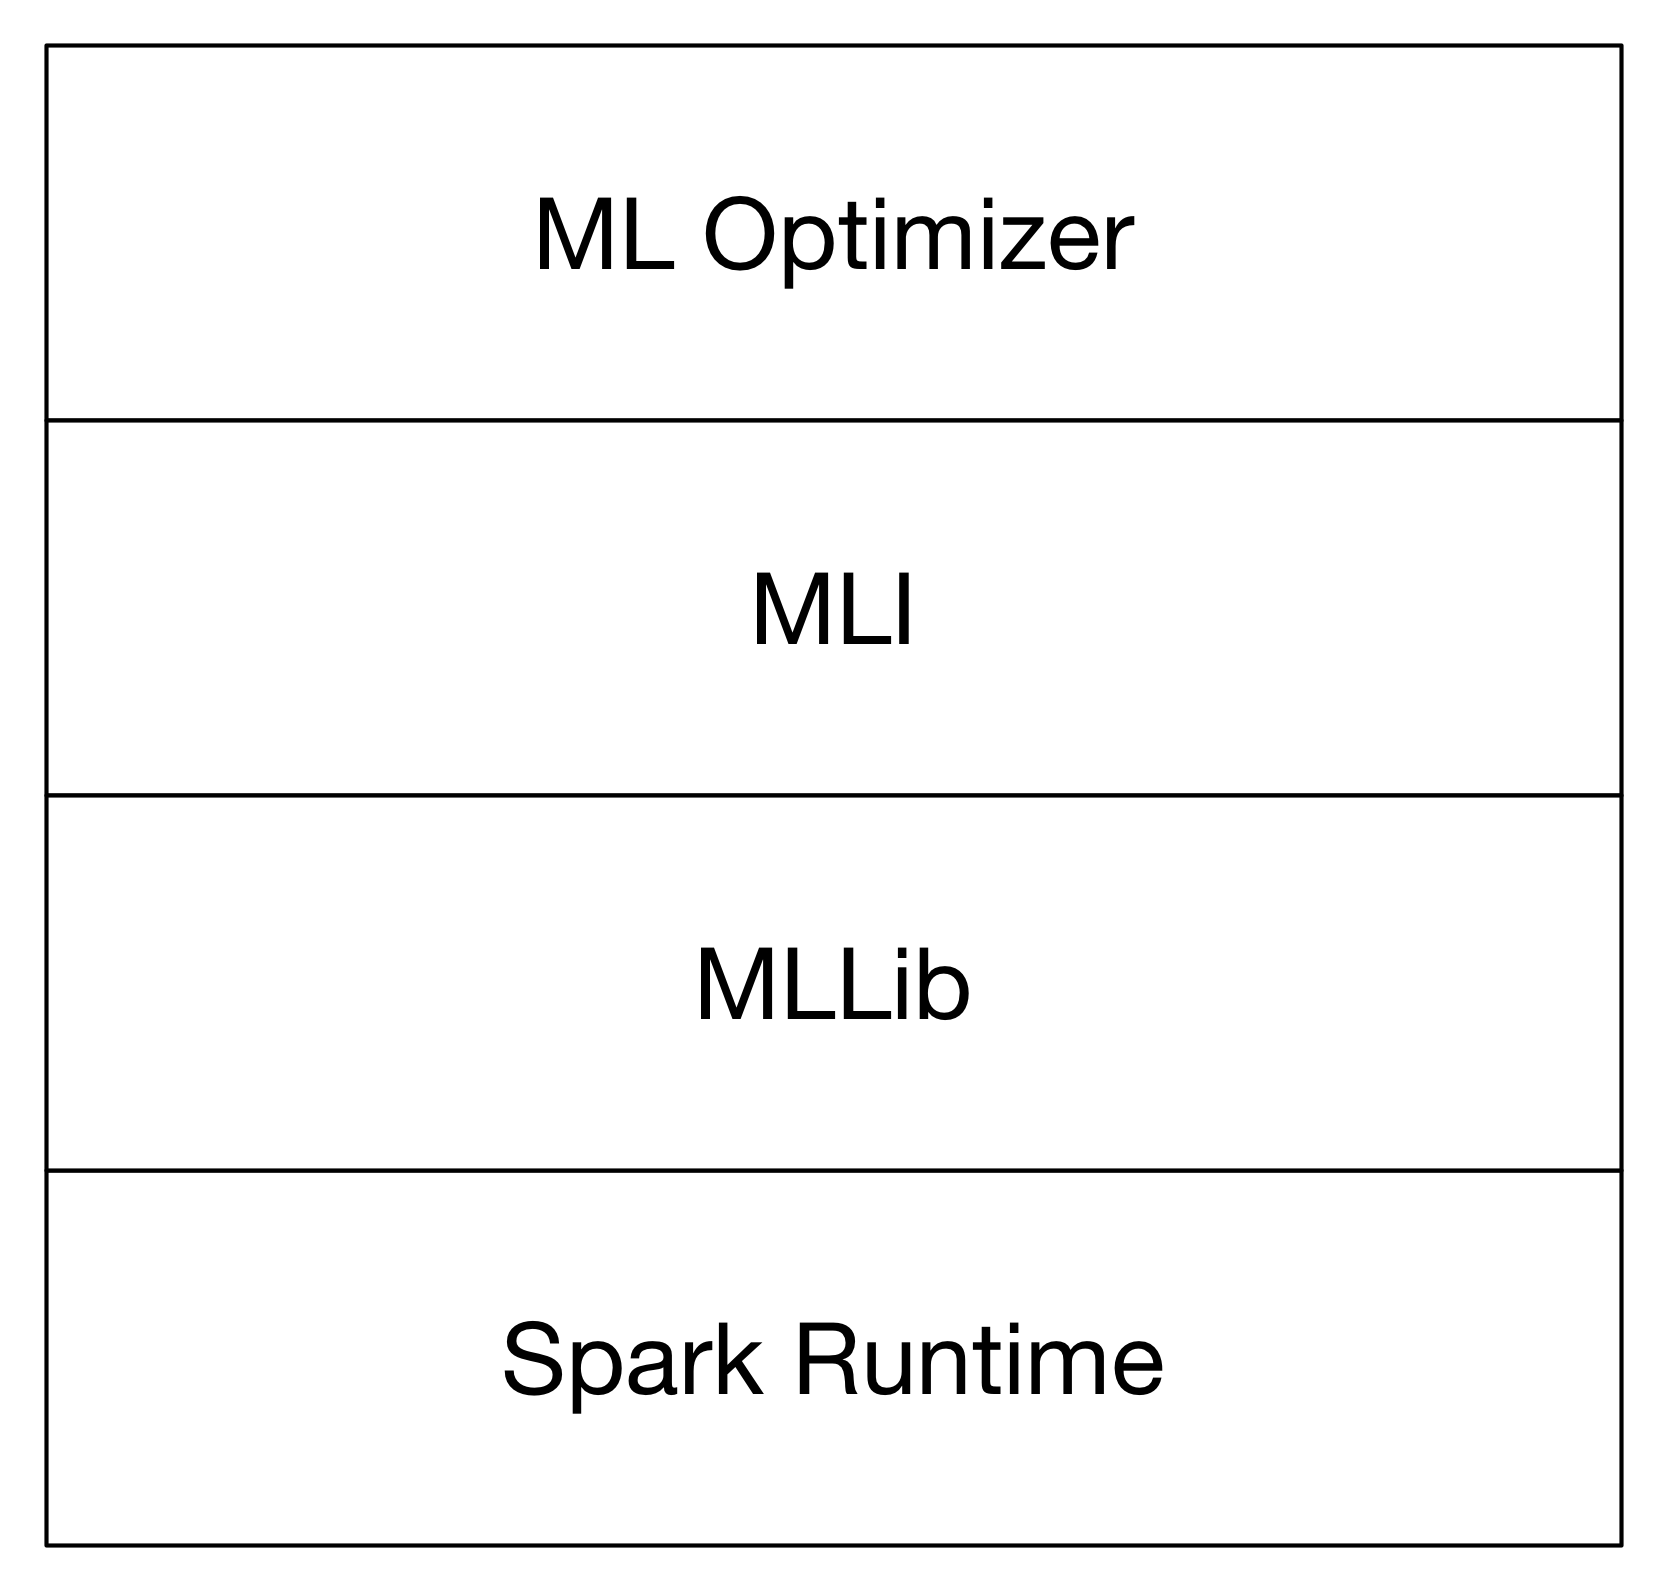
\includegraphics[width=0.5\textwidth]{bilder/2_4_3_mlbase.png}
\caption{Die Bestandteile der MLbase }
\label{fig:mlbase}
\end{figure} 
 


Die MLlib ist eine verteilte Machine-Learning-Bibliothek die für die Spark-Laufzeitumgebung entwickelt wurde und die bekannten Algorithmen für Probleme wie Klassifikation, Regression, Clustering und kollaboratives Filtern enthält (Vergleich \citeint{ml10}).

Bei MLI handelt es sich um eine API, die es ermöglicht, selbst ML-Features zu entwickeln und in erster Linie für komplexere Problemstellungen geeignet ist. Mit MLI lassen sich die Funktionen direkt gegen Spark entwickeln, gegebenenfalls unter Zuhilfenahme der Bibliotheken der MLlib.

Der ML-Optimizer soll ML-Probleme für Endnutzer vereinfachen, in dem Modellauswahlen automatisiert werden. Hierzu werden Features aus der MLlib und der MLI extrahiert und zur Hilfe genommen.



\section{Spark SQL}
\label{section:spark SQL}


Im Ökosystem von Hadoop ist Hive \textit{Hive} ist eine \textit{SQL-Query-Engine} , die sich großer Beliebtheit in der Community erfreut und trotz zahlreich  Spark SQL\footnote{Ursprünglich war die für den BDAS-Stack empfohlene Implementierung einer SQL-Query-Engine unter dem Namen \textit{Shark} bekannt. Im Juli 2014 wurde jedoch bekanntgegeben, dass die Entwicklung von Shark zugunsten von Spark SQL eingestellt wurde und die vorhandenen Shark-Implementierungen voll in Spark SQL integriert werden. Deshalb zeigen Schaubilder des BDAS von vor Juli 2014 Shark als Query-Engine.} ist eine Portierung dieser Engine für Spark, um alle Vorteile der BDAS-Architektur nutzen zu können und ist kompatibel mit sämtlichen Hive-Daten, -Metastores und –Queries. Im Gegensatz zu Hive, das aus Datensätzen zur Laufzeit Java-Objekte generiert, nutzt Spark SQL eine zeilenorientierte Speicherung mittels Arrays primitiver Datentypen und ist somit selbst in einer Hadoop-Infrastruktur im Mittel bis zu fünfmal schneller als Hive. 

Eine Besonderheit von Spark SQL ist neben seinem SQL-Interface die Möglichkeit, auch Machine-Learning-Funktionen als Abfragen formulieren zu können. 

Für die Anwendung von Spark SQL hat sich die Architektur von Spark mit seinen RDDs als sehr vorteilhaft erwiesen, da Abfragen auf Fehlerhaften RDDs nach dem Neuaufbau des entsprechenden Datasets direkt erneut ausgeführt werden können. 

Ein weiterer Unterschied zu Hive ist die sogenannte Partial-DAG-Execution (PDE). Dies bedeutet, dass logische Abfragepläne in Spark SQL aufgrund gesammelter Statistiken zur Laufzeit flexibel erstellt werden im Gegensatz zu Hive oder herkömmlichen relationalen Datenbanksystemen, wo bereits zur Kompilierungszeit starre physische Abfragepläne generiert werden. Besonders die Machine-Learning- und Failover-Funktionen wären mit einer Planerstellung zu Kompilierzeit nicht umsetzbar. 






\section{Zusammenfassung}
\label{section:zusammen}



TBD!
